\documentclass[11pt,a4paper]{article}
\usepackage[T1]{fontenc}
\usepackage[utf8]{inputenc}
\usepackage{lmodern,amsmath,amssymb,booktabs,graphicx,longtable,geometry,hyperref,array,microtype,needspace}
\geometry{margin=25mm}
\hypersetup{colorlinks=true,linkcolor=blue,urlcolor=blue,citecolor=blue,pdfauthor={Russlan Ramdowar},pdftitle={Ranking AI Investment Forecasts}}
\numberwithin{table}{section}
\setlength{\emergencystretch}{3em}
\renewenvironment{abstract}{\small\noindent\textbf{Abstract}\par\medskip}{\par}
\setlength{\parskip}{.4em}
\setlength{\parindent}{0pt}
\newcommand{\clip}{\operatorname{clip}}
\newcommand{\G}{\operatorname{G10}}
\title{Ranking AI Investment Forecasts: Original Scoring, Dynamic Rescoring, and the Trade-Off Between Return-Focused and Risk-Adjusted Strategies}
\author{Russlan Ramdowar\\Future Edge Group FZE / iPulse AI\\\href{mailto:russlan@ipulseai.com}{russlan@ipulseai.com}}
\date{Completed research manuscript --- 4 November 2026}
\begin{document}
\maketitle
\vspace{-1.1em}
\begin{abstract}

Investment platforms powered by artificial intelligence face two distinct ranking decisions that are almost universally conflated: how to score a newly generated forecast at inception, and how to update that ranking as market prices move between deep research cycles. At the same time, ranking design must distinguish between investors seeking maximum upside and those seeking protection against historical volatility. To resolve both questions empirically, we conduct two large-scale portfolio studies alongside a controlled bridge to our companion research-reuse framework (Ramdowar, 2026). First, an original-scoring study evaluates 48 fixed formula configurations across six stock cohorts, three portfolio sizes (Top 10, 20, and 30), two allocation schemes, and two entry conventions, spanning 3,456 portfolios held through 2 November 2026. Second, an independent rescoring study evaluates 115 repricing policies at 7-, 14-, and 30-day checkpoints across one-year and five-year forecast selections and Top 10/20 equal-weight portfolios, spanning 8,280 portfolios held through 3 November 2026. Every portfolio begins with USD 100,000 and tracks actual gross distributions, corporate actions, and foreign exchange through its frozen valuation cutoff. Three core findings emerge:

\textbf{Objective Separation at Inception:}  Our Return-Focused (G10) formula---which balances expected excess return against ensemble forecast disagreement and dispersion---ties for the strongest Top 10 equal-weight return midrank across all 48 candidates. Meanwhile, a clean Risk-Adjusted (B02) ratio of forecast excess return to historical price volatility delivers the strongest return-to-drawdown profile among all 27 volatility-aware rules, reducing drawdowns in all 12 matched Top 20 cohort-entry cells relative to the legacy core.

\textbf{Conviction Continuity Beats Shock Penalties in 1-Year Rescoring:}  Testing 108 price-shock haircut rules reveals that penalizing stocks after interim price moves fails to improve performance. Instead, a 75/25 continuity blend---combining 75\% of the fixed original G10 score with 25\% of the price-updated G10 score under current BUY eligibility guards---outperforms raw updated G10 in 15 of 18 primary matched cells (raising descriptive mean return from 12.80\% to 19.54\%) and 25 of 36 cells across all six cohorts (raising mean return from 7.78\% to 14.70\%). For five-year selections, raw updated G10 is retained because the blend wins fewer than half the matched cells, despite having a higher mean return.

\textbf{Synergy with Research Reuse:}  Extending the 75/25 continuity blend to the 203-stock panel from our companion study (Ramdowar, 2026) yields an additional 1.23 percentage points of net Top 10 return over raw G10 across unchanged-model short windows (6.19\% vs. 4.96\%, and 0.67 percentage points after removing each portfolio's single best winner). However, broader Top 30 portfolios and extended holding windows expose clear limits to score blending when underlying fundamentals grow stale.

Based on this evidence, we adopt G10 as the principal Return-Focused engine, implement the 75/25 continuity blend for one-year BUY rescoring, retain raw updated G10 for five-year and non-BUY rescoring, and maintain B02 as a dedicated Risk-Adjusted strategy. Methodological boundaries, outlier sensitivities, and retrospective backtesting limitations are consolidated in Section 10.

\textbf{Observation Cutoffs:}  Original-scoring portfolios end on 2 November 2026; rescoring portfolios end on 3 November 2026. The two studies are evaluated and reported as separate experimental records.

\end{abstract}
\clearpage
\tableofcontents
\clearpage
\section{The Core Dilemma: Scoring New Research vs. Repricing Existing Conviction}

When an AI investment committee finishes a deep, multi-agent analysis of a company, it produces a rich set of forecasts: expected price targets, dividend assumptions, and measures of agreement or dispersion across participating analytical models. Ranking stocks at that moment of creation is a problem of original scoring. Days or weeks later, however, market prices have moved while the underlying research report remains unchanged. If a stock's price drops 10\% two weeks after a bullish forecast, its mechanical upside to the original target price rises---yet the market move might also signal headwinds. Conversely, if the stock rallies 15\%, its remaining mathematical upside shrinks, even though the market is validating the bullish thesis. Deciding how to re-order existing forecasts as prices fluctuate---without commissioning a fresh multi-agent research run---is the problem of dynamic rescoring. Most quantitative ranking systems treat original scoring and daily rescoring as the same operation, simply plugging today's stock price into the original formula. Worse, many systems try to force a single ranking score to satisfy two incompatible investor temperaments: maximizing total return (which requires tolerating concentration and volatility to capture multi-bagger outliers) and minimizing drawdowns (which requires penalizing historically volatile stocks even when their expected upside is high). This study resolves both tensions by separating when a forecast is scored from what investment objective the score serves. Following a comprehensive evaluation of 11,736 simulated portfolios across two dedicated experiments, we establish the Version 8 (V8) operating policy for the iPulse AI platform:

\textbf{Principal Return-Focused Strategy (G10):}  Designed for investors prioritizing capital appreciation. At inception, G10 ranks stocks using expected excess return tempered by two ensemble disagreement penalties (mean absolute forecast deviation and forecast standard deviation). During daily rescoring of eligible one-year BUY candidates, the system applies a 75/25 continuity blend---combining 75\% of the fixed original G10 score with 25\% of the price-updated G10 score---while five-year rankings and non-BUY candidates continue to use raw price-updated G10.

\textbf{Dedicated Risk-Adjusted Strategy (B02):}  Designed for investors prioritizing smoother equity curves and shallower drawdowns. Both at inception and during rescoring, B02 ranks eligible candidates by dividing forecast excess return by historical price volatility, without score blending.

\textbf{Portfolio Breadth Alignment:}  Because return-seeking and risk-conscious strategies behave differently under concentration, our primary research constructions pair Return-Focused G10 with concentrated Top 10 equal-weight portfolios and Risk-Adjusted B02 with broader Top 20 equal-weight portfolios, while reporting matched Top 10 comparisons to isolate formula mechanics from portfolio breadth.

\begin{minipage}{\linewidth}
\begin{center}\small\setlength{\tabcolsep}{3pt}\renewcommand{\arraystretch}{1.18}
\begin{longtable}{@{}p{.19\linewidth}p{.32\linewidth}p{.42\linewidth}@{}}
\caption{Original scoring and dynamic rescoring policies}\\
\toprule
Strategy dimension & Original scoring & Dynamic rescoring\\\midrule\endhead
Return-Focused (G10) & G10 computed on frozen original forecast inputs & 1Y BUY: 75\% fixed original G10 + 25\% updated G10 blend; 5Y \& non-BUY: Raw updated G10\\
Risk-Adjusted (B02) & B02 ratio: forecast excess return divided by historical volatility & B02 computed on checkpoint remaining return and checkpoint historical volatility (no continuity blend)\\
Evaluated Portfolio Grid & Top 10, Top 20, and Top 30; equal or linearly declining weights & Top 10 and Top 20; equal weights at each independent checkpoint entry\\
\bottomrule\end{longtable}\end{center}
\end{minipage}\par
Crucially, elevating G10 to the principal ranking and retaining B02 as a dedicated alternative reflects an explicit alignment of product objectives rather than a claim that one formula is universally superior in all market environments. Earlier internal drafts proposed B02 as the public default under a capital-resilience mandate; when the platform's primary mandate was clarified to prioritize upside capture while offering risk-adjusted screening as a distinct choice, G10 became the principal engine and B02 the dedicated risk-adjusted screen. Calling these strategies "Return-Focused" and "Risk-Adjusted" replaces our preliminary labels (Risk Accepting and Risk Balancing) with transparent descriptions of what the mathematics actually do.

\section{Experimental Architecture: Two Distinct Studies, 11,736 Portfolios}

To prevent data leakage between initial formula design and post-entry repricing, we structured our investigation as two separate experiments with distinct entry clocks, eligibility rules, risk-input lineages, and frozen valuation cutoffs.

\subsection{The Original-Scoring Experiment (3,456 Portfolios)}

Our original-scoring investigation progressed through three cumulative stages---an initial 7-rule pilot, a 40-rule factorial development study, and a final 8-rule mechanism extension---all of which are retained in full so that failed variants remain just as visible as winning ones. The core 40-rule grid comprises a complete $2^5$ factorial (32 combinations) toggling five building blocks---historical price volatility ($V$), mean absolute forecast disagreement ($M$), directional consistency ($A$), forecast dispersion ($D$), and a 20\% five-year horizon blend ($H$)---augmented by 8 benchmark reference rules and 8 targeted mechanism checks, yielding 48 total configurations. We evaluate all 48 configurations across six historical forecast cohorts (Batches 1--6) comprising 1,505 stock--batch pairs (3,010 total horizon rows across 1-year and 5-year forecasts). To isolate pure ranking order without survivorship or selection bias, every cohort retains its complete universe of stocks without filtering on current active status or historical BUY labels. Because historical scores in early platform cohorts were back-populated into the compatible v2.3 database schema in June 2026, we evaluate every portfolio under two distinct entry conventions:

\textbf{Retrospective Original-Anchor Entry:}  Enters at the original forecast anchor date (a counterfactual measuring how formulas would have performed if v2.3 scores had been live at the moment of forecast generation).

\textbf{Source-Availability Entry:}  Waits to enter until the exact timestamp when compatible stored scores existed in the database.

\begin{minipage}{\linewidth}
\begin{center}\small\setlength{\tabcolsep}{3pt}\renewcommand{\arraystretch}{1.18}
\begin{longtable}{@{}lrrr@{}}
\caption{Forecast cohorts and compatible score availability}\\
\toprule
Batch & Forecast anchor & Stocks & Score availability\\\midrule\endhead
Batch 1 & 28 Nov 2025 & 184 & 25 Jun 2026\\
Batch 2 & 19 Mar 2026 & 190 & 25 Jun 2026\\
Batch 3 & 11 Apr 2026 & 217 & 25 Jun 2026\\
Batch 4 & 3 May 2026 & 283 & 25 Jun 2026\\
Batch 5 & 5 Jun 2026 & 283 & 15 Jun 2026\\
Batch 6 & 5 Jul 2026 & 348 & 6 Jul 2026\\
\bottomrule\end{longtable}\end{center}
\end{minipage}\par
Across the 48 formulas, 6 cohorts, 3 portfolio sizes (Top 10, Top 20, Top 30), 2 weighting schemes (equal weights and linearly declining rank weights), and 2 entry conventions, the original-scoring matrix encompasses $48 \times 6 \times 3 \times 2 \times 2 = \mathbf{3,456\text{ portfolios}}$. Each portfolio starts with USD 100,000 and remains invested on a strict buy-and-hold basis until 2 November 2026.

\subsection{The Dynamic Rescoring Experiment (8,280 Portfolios)}

Once a forecast cohort is published, how should an investor or platform rank those stocks 7, 14, or 30 calendar days later after market prices have shifted? Our second experiment tests 115 rescoring policies across those three post-anchor checkpoints. Each checkpoint is evaluated at UTC end-of-day using only dated local closing prices and corporate actions known on or before that date, entering at the next available local market open with a fresh USD 100,000 allocation held through 3 November 2026. The rescoring policy design unfolded in two stages:

\textbf{Round 1 (58 Policies --- Return-Level Shock Haircuts):}  Combined 4 baseline references with 54 return-shrinkage rules that penalize remaining expected return when a stock's price deviates sharply from its expected geometric path.

\textbf{Round 2 (57 Additional Policies --- Score-Level Haircuts \& Continuity Blends):}  After observing that return-level haircuts often failed to dislodge extreme outliers due to hyperbolic tangent ($\tanh$) saturation in G10, we added 54 score-level shock haircuts (which directly scale down the G10 score) alongside 3 original/current score continuity blends (weighting the original G10 score at 25\%, 50\%, and 75\%). Evaluating all 115 policies across 6 cohorts, 3 checkpoint lags (7, 14, and 30 days), 2 selection horizons (1Y and 5Y forecast rankings), and 2 equal-weight portfolio breadths (Top 10 and Top 20) produces $115 \times 6 \times 3 \times 2 \times 2 = \mathbf{8,280\text{ portfolios}}$ built from 9,024 risk-comparable asset--horizon--checkpoint records.

To ensure practical deployability, our primary rescoring tables apply the platform's live economic BUY eligibility screen at each checkpoint:Remaining annualized expected total return must be at least 3.6\%.Remaining expected return minus original mean absolute disagreement ($R_t - M_0$) must be at least $-1.0$ percentage point. Current raw updated G10 must exceed 130 (and any G10-derived variant must also exceed 130 on its own score, while B02 ranks the eligible BUY universe by its volatility-adjusted ratio). Even at the most restrictive checkpoint, at least 23 stocks pass the BUY screen, ensuring every Top 10 and Top 20 portfolio is 100\% invested in qualifying equities without silent cash dilution.

\subsection{Why the Two Experiments Must Remain Separate}

Although both experiments evaluate G10 and B02, their underlying portfolios cannot be merged into a single return series. They differ across four structural dimensions: entry dates (anchor/availability vs. +7/+14/+30 day checkpoints), universe filtering (unfiltered cohorts vs. current BUY eligibility screens), historical volatility inputs (legacy raw-close series vs. dated corporate-action-adjusted return series), and terminal valuation cutoffs (2 November vs. 3 November 2026). All strategy comparisons are therefore conducted strictly within matched experimental cells.

\section{Original Scoring: Mathematical Formulation of G10 and B02}

A sound ranking formula must translate ensemble AI predictions into a bounded, monotone score without obscuring the economic trade-off between expected return, model disagreement, and market volatility. Below, all return and volatility variables are expressed in percentage points.

\subsection{Return-Focused G10}

For any stock and forecast horizon, let $R$ denote the annualized expected total return (incorporating the original eligible dividend yield assumption), $M$ denote the mean absolute deviation of individual model forecasts around their arithmetic mean (distinct from median absolute deviation), and $s$ denote the standard deviation of those model forecasts. G10 is computed in five sequential steps:

\begin{equation}e = R - 3.6 \end{equation}

\begin{equation}E = \operatorname{sgn}(e)\Big(|e| - \min(0.35M,\, 0.60|e|)\Big) \end{equation}

\begin{equation}b = \min\Big(10,\, \max(1,\, 0.5|R|)\Big) \end{equation}

\begin{equation}P = 0.15\min\left(1,\, \left[\frac{\max(0,\, s - b)}{\max(15 - b,\, 1)}\right]^2\right) \end{equation}

\begin{equation}\operatorname{G10}(R, M, s) = 1000\tanh(E / 30)(1 - P) \end{equation}

where $E = 0$ whenever $e = 0$.

Each step in G10 serves a clear economic purpose:

\textbf{Hurdle Subtraction (Eq. 1):}  Deducts a fixed 3.6 percentage-point baseline hurdle to center excess return $e$.

\textbf{Bounded Disagreement Discount (Eq. 2):}  Penalizes excess return by $0.35M$ to reflect ensemble uncertainty, but caps that penalty at 60\% of $|e|$ so that a high-upside stock with wide analyst debate retains its positive directional sign rather than flipping negative.

\textbf{Proportional Dispersion Allowance (Eqs. 3--4):}  Defines a "normal dispersion buffer" $b$ that scales with return magnitude (between 1 and 10 percentage points). Only forecast standard deviation $s$ exceeding $b$ triggers the quadratic penalty $P$, which trims the final score by at most 15\% ($1 - P \in [0.85, 1.00]$).

\textbf{Saturating S-Curve Mapping (Eq. 5):}  Passing $E/30$ through $\tanh(\cdot)$ maps scores smoothly into $(-1000, 1000)$, preventing extreme price targets from dominating portfolio selection linearly while preserving full-precision ranking order (with deterministic subject-ID tie-breaking prior to display rounding).

Notably, G10 deliberately excludes historical stock-price volatility, event-risk flags, directional vote-consistency multipliers, and cross-horizon blends. It is a pure conviction-and-upside engine: it penalizes internal disagreement among AI models, but it does not penalize a stock for having a volatile market history.

\subsection{Risk-Adjusted B02}

Investors who want protection against turbulent market swings need an explicit historical volatility normalizer. Why not rely on G10's disagreement penalties ($M$ and $s$) to control risk? Because model disagreement and market price volatility are fundamentally different phenomena: an AI ensemble can agree tightly on the target price of a highly volatile biotech stock, or disagree widely on the valuation of a stable utility company.

To normalize explicitly for market turbulence, let $v$ represent the stock's annualized historical price volatility (computed over a ten-year lookback requiring at least 60 daily return observations, floored at 5 percentage points to prevent near-zero denominators). Risk-Adjusted B02 ranks candidates by the ratio:

\begin{equation}J = \frac{R - 3.6}{\max(v,\, 5)} \end{equation}

For platform display, $J$ can be mapped through the strictly monotone transformation $1000\tanh(J/2)$, which leaves ranking order untouched. Unlike complex composite rules that mix volatility with disagreement and multi-horizon terms, B02 strips away all secondary multipliers to answer a single, transparent question: how much expected excess return does this forecast offer per unit of historical price volatility?

\section{Original-Scoring Evidence: Why Simplicity and Objective Separation Win}

Evaluating all 48 candidate formulas across 3,456 portfolios reveals a striking lesson in quantitative design: focused, single-purpose formulas outperform complex hybrids, and separating return maximization from drawdown control is superior to forcing a compromise.

\textbf{G10 Leads on Upside Rank:}  Across all six cohorts and both entry conventions, G10 ties for the best (lowest) average Top 10 equal-weight return midrank among all 48 formulas: 15.83 under original-anchor entry and 17.83 under source-availability entry. The only formula that ties G10 is HNEG (a complex variant that shrinks negative 1Y scores toward zero when the 5Y score is negative), which ties solely because its modification affects negative-scoring stocks and therefore produces the exact same Top 10 BUY selections as G10. By Occam's razor, G10 captures the full return advantage without unnecessary complexity.

\textbf{B02 Leads on Drawdown Resilience:}  Among the 27 candidate rules that incorporate historical price volatility, B02 achieves the best aggregate return-to-drawdown midrank across all portfolio constructions: 9.56 at anchor entry and 9.14 at source availability. In head-to-head comparisons at matched Top 20 equal-weight breadth against the platform's legacy stored core (B03), B02 achieves a shallower maximum drawdown in all 12 out of 12 cohort-entry cases, a higher return-to-drawdown ratio in 9 of 12 cases, and a higher raw return in 7 of 12 cases.

\subsection{Retrospective Original-Anchor Entry (End Date: 2 November 2026)}

\begin{minipage}{\linewidth}
\begin{center}\small\setlength{\tabcolsep}{3pt}\renewcommand{\arraystretch}{1.18}
\begin{longtable}{@{}lrrrrrr@{}}
\caption{Original-anchor returns and maximum drawdowns (\%)}\\
\toprule
Batch & G10/10 R & G10/10 DD & B02/10 R & B02/10 DD & B02/20 R & B02/20 DD\\\midrule\endhead
Batch 1 & 48.39 & -24.45 & 23.50 & -16.32 & 50.53 & -8.81\\
Batch 2 & 37.12 & -11.78 & 9.88 & -6.77 & 12.89 & -5.29\\
Batch 3 & 25.65 & -13.11 & 8.71 & -8.25 & 16.81 & -7.38\\
Batch 4 & 52.95 & -13.32 & 9.42 & -10.02 & 14.90 & -7.10\\
Batch 5 & 13.37 & -14.58 & 6.49 & -13.71 & 7.13 & -10.84\\
Batch 6 & 10.19 & -17.63 & 13.05 & -14.75 & 11.79 & -9.85\\
\bottomrule\end{longtable}\end{center}
\end{minipage}\par
Note: $R$ denotes total holding-period return (\%) and $DD$ denotes signed maximum drawdown (\%) through 2 November 2026 under equal weighting.

\subsection{Later Source-Availability Entry (End Date: 2 November 2026)}

\begin{minipage}{\linewidth}
\begin{center}\small\setlength{\tabcolsep}{3pt}\renewcommand{\arraystretch}{1.18}
\begin{longtable}{@{}lrrrrrr@{}}
\caption{Source-availability returns and maximum drawdowns (\%)}\\
\toprule
Batch & G10/10 R & G10/10 DD & B02/10 R & B02/10 DD & B02/20 R & B02/20 DD\\\midrule\endhead
Batch 1 & 5.57 & -20.22 & 8.35 & -7.17 & 22.07 & -4.29\\
Batch 2 & 25.36 & -11.58 & 9.14 & -6.74 & 7.14 & -5.63\\
Batch 3 & 12.66 & -10.94 & 10.73 & -8.63 & 8.48 & -8.26\\
Batch 4 & 47.41 & -8.24 & 17.28 & -9.85 & 21.59 & -6.83\\
Batch 5 & 17.18 & -14.52 & 8.47 & -13.69 & 7.47 & -10.77\\
Batch 6 & 7.45 & -17.62 & 11.55 & -14.74 & 9.68 & -9.90\\
\bottomrule\end{longtable}\end{center}
\end{minipage}\par
(See Figure 1 in the companion figure archive for a visual bar-chart comparison of G10 vs. B02 returns and maximum drawdowns across Batches 1--6 at matched Top 10 equal breadth.)
\begin{figure}[!ht]\centering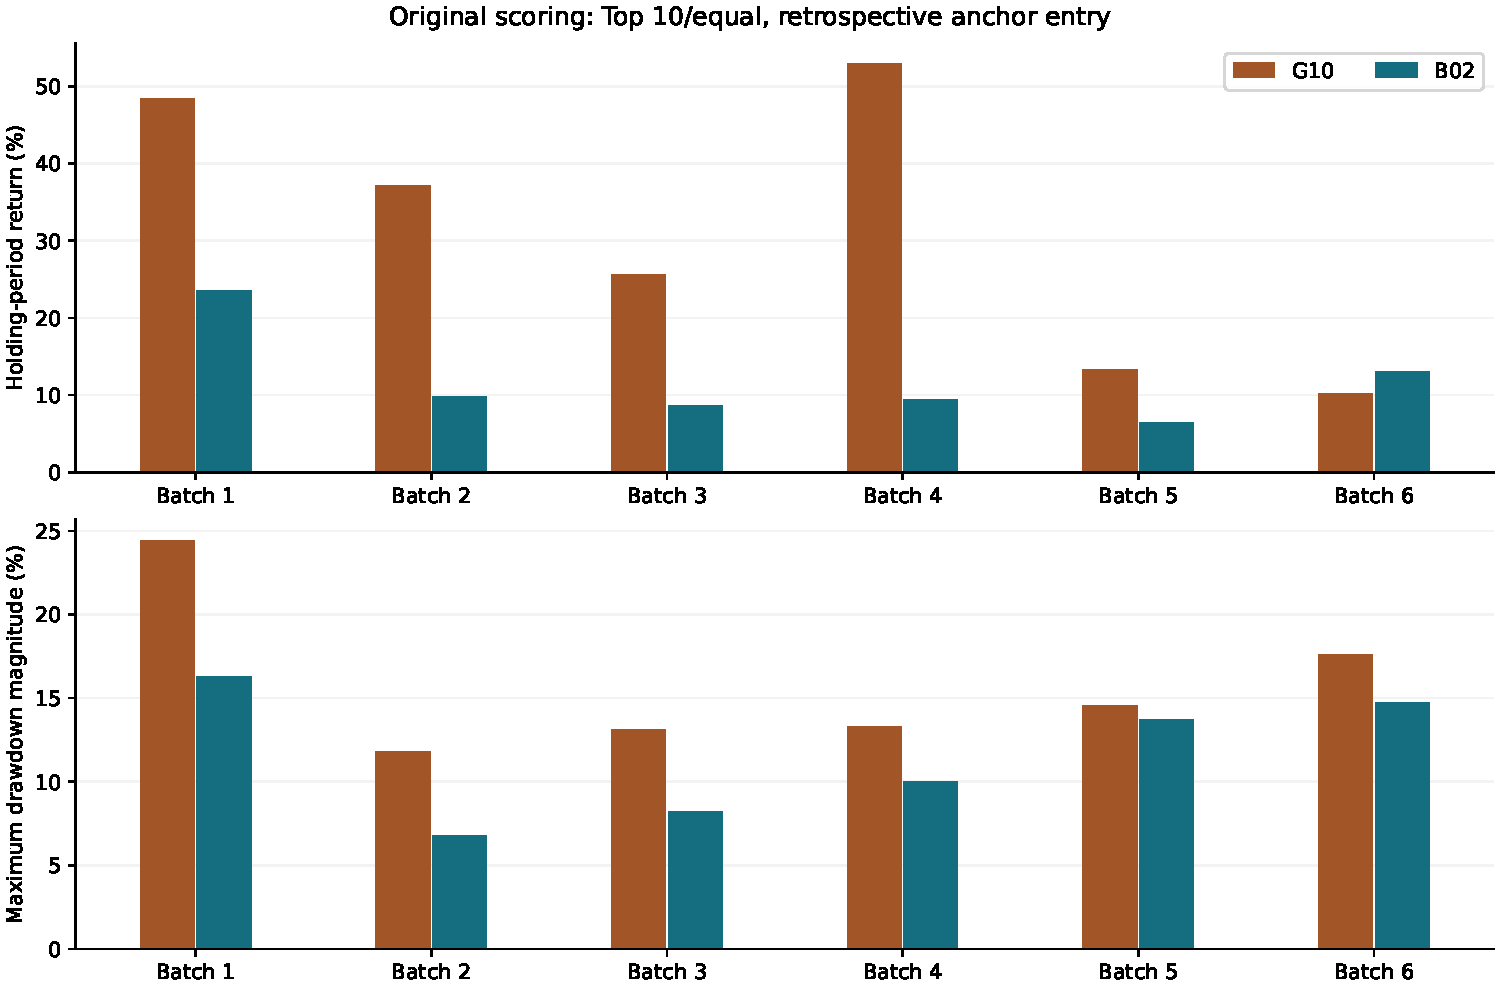
\includegraphics[width=.97\linewidth]{original_comparison.pdf}\caption{Original scoring: matched Top 10 equal-weight portfolios across six cohorts, original-anchor entry.}\end{figure}

\subsection{Isolating Individual Formula Components ($2^5$ Factorial Analysis)}

Because our 32-rule core forms a balanced $2^5$ factorial, we can isolate the average marginal effect of switching each of the five formula components ON versus OFF across 576 matched portfolio pairs (spanning 6 cohorts and 6 breadth/weighting constructions):

\begin{minipage}{\linewidth}
\begin{center}\small\setlength{\tabcolsep}{3pt}\renewcommand{\arraystretch}{1.18}
\begin{longtable}{@{}lrrrr@{}}
\caption{Factorial component effects (percentage points)}\\
\toprule
Component & Anchor R & DD gain & Available R & DD gain\\\midrule\endhead
Volatility Bundle ($V$) & -2.88 & +4.31 & -0.64 & +1.92\\
Mean Disagreement ($M$) & -0.46 & +0.52 & +0.43 & +0.21\\
Directional Consistency ($A$) & -0.14 & +0.13 & -0.13 & +0.01\\
Forecast Dispersion ($D$) & +0.13 & +0.76 & +0.44 & +0.22\\
Five-Year Blend ($H$) & -0.37 & -0.32 & -0.18 & -0.19\\
\bottomrule\end{longtable}\end{center}
\end{minipage}\par
Note: Positive Drawdown Gain (pp) indicates a shallower (improved) maximum drawdown.

The factorial decomposition makes the design trade-offs unmistakable:

\textbf{The Volatility Trade-Off ($V$):}  Turning on historical volatility normalization improves maximum drawdown substantially (+4.31 pp at anchor entry, +1.92 pp at availability) but costs raw upside (-2.88 pp at anchor, -0.64 pp at availability). That sharp divergence is precisely why volatility belongs in a dedicated Risk-Adjusted strategy (B02) rather than inside the Return-Focused engine (G10).

\textbf{Ensemble Dispersion \& Disagreement ($D$ and $M$):}  Forecast dispersion ($D$) improves both average return and drawdown under both entry conventions. Mean disagreement ($M$) consistently reduces drawdown (+0.52 pp and +0.21 pp) and improves return under source-availability entry (+0.43 pp). Both are retained in G10.

\textbf{Why Consistency ($A$) and 5Y Blending ($H$) Were Dropped:}  Adding a separate directional-consistency multiplier ($A$) slightly reduces returns with negligible drawdown benefit, while blending 20\% of the 5-year score into the 1-year score ($H$) degrades both average return and average drawdown under both entry modes.

\subsection{Separating the archived volatility mechanisms}

The archive allows the volatility trade-off to be examined more closely.
A00 adds only the softer volatility denominator to G10; G26 switches on
the full volatility bundle while retaining G10's disagreement settings;
B02 uses the pure excess-return/volatility ratio. Across the 36 matched
cohort, breadth and allocation constructions under each entry convention,
their differences from G10 are:

\begin{minipage}{\linewidth}
\begin{center}\small\setlength{\tabcolsep}{4pt}\renewcommand{\arraystretch}{1.18}
\begin{longtable}{@{}lrrrr@{}}\toprule
Rule & Anchor R pp & Anchor DD gain & Available R pp & Available DD gain\\\midrule\endhead
A00 & -0.49 & +1.21 & +0.04 & +0.53\\
G26 & -4.51 & +3.71 & -1.80 & +1.61\\
B02 & -6.17 & +4.99 & -1.82 & +3.14\\
\bottomrule\end{longtable}\end{center}
\end{minipage}\par

A00 preserves more upside while providing a modest drawdown improvement.
B02 makes the stronger risk-objective trade: its average drawdown gain is
4.99 percentage points at anchor entry and 3.14 points at availability,
compared with 3.71 and 1.61 points for the bundled G26 rule. The profiles
also differ in design: A00's denominator rises only to 1.25, versus 2.0
inside the full bundle, and B02 omits the ensemble-disagreement penalties.
This comparison explains the separate roles of the simple return-focused
and volatility-adjusted screens.


\section{Dynamic Rescoring: Repricing Forecasts Without New AI Inference}

Between deep research refreshes, how should an investment system update its rankings as market prices move?

\subsection{Repricing Remaining Expected Return ($R_t$)}

Let $P_0$ denote the stock's split-adjusted closing price at the original forecast anchor, $P_t$ denote the dated local closing price at checkpoint $t$ (7, 14, or 30 days later), $T$ denote the frozen price-only terminal target from the original forecast, and $\tau_t$ denote the remaining years to horizon expiry. Keeping the original annual dividend yield assumption $y_0$ fixed per share (so that a change in share price scales the effective dividend yield by $P_0 / P_t$), the updated annualized expected total return $R_t$ (in percentage points) is:

\begin{equation}R_t = 100\left[\left(\frac{T}{P_t}\right)^{1/\tau_t}\left(1 + y_0\frac{P_0}{P_t}\right) - 1\right] \end{equation}

During rescoring, the original ensemble disagreement ($M_0$) and dispersion ($s_0$) statistics remain frozen. Feeding $(R_t, M_0, s_0)$ directly into Equation 5 yields Raw Updated G10: a purely mechanical repricing that treats any stock drop as higher remaining upside and any stock rally as lower remaining upside.

\subsection{Testing Two Competing Hypotheses: "Price-Shock Haircuts" vs. "Conviction Continuity"}

Pure mechanical repricing raises an obvious concern: what if a large price move after forecast publication means the market knows something the AI forecast missed, or that the move has already exhausted the thesis? Conversely, what if mechanical repricing overreacts to routine short-term market noise, prematurely selling winners that have started to rally and rotating into lagging stocks?

We tested both hypotheses systematically across 115 policies:

\textbf{The Price-Shock Haircut Family (108 Policies):} We measure a stock's interim price shock against its geometric expected trajectory $P_0(T/P_0)^f$, where $f$ is the elapsed fraction of the forecast horizon. Using the checkpoint's preceding action-adjusted daily volatility $v_t$, we define a volatility-scaled threshold $q = \operatorname{clip}(\max(v_t, 5)\sqrt{\Delta t},\, 8,\, 20)$ percentage points and apply a cubic smoothstep function $u(x) = z^2(3 - 2z)$ with $z = \operatorname{clip}((x - a)/(b - a),\, 0,\, 1)$ across stated start/full gates $(a, b)$. Whenever a signed price shock passes the tested direction and gate, a penalty weight $w$ is set to the policy cap multiplied by the larger of the smoothstep on $|\text{shock}|/q$ over $[0.75, 1.50]$ and the smoothstep on absolute shock over $(a, b)$.We tested 54 return-level shock rules---which shrink excess return via $R_t' = 3.6 + (1 - w)(R_t - 3.6)$ before computing G10---and 54 score-level shock rules---which directly shrink the resulting score via $\operatorname{G10}(R_t, M_0, s_0)(1 - w)$---spanning six maximum penalty caps $\{0.20, 0.35, 0.50, 0.75, 0.90, 1.00\}$, three absolute start/full gate pairs $\{(8, 20), (12, 25), (20, 40)\}$, and three shock directions (both directions, downward shocks only, and upward shocks only), plus the legacy V7 shock reference (which used caps of 0.50 for 1Y and 0.20 for 5Y on the older V7 core).

\textbf{The Conviction Continuity Family (3 Blend Policies + 2 Endpoint Controls):} Rather than penalizing interim price volatility, the continuity family anchors the updated ranking to the original inception conviction score while allowing current market pricing to exert a bounded pull:

\begin{equation}S_t(\lambda) = \lambda\operatorname{G10}(R_0, M_0, s_0) + (1 - \lambda)\operatorname{G10}(R_t, M_0, s_0), \quad \lambda \in \{0.25, 0.50, 0.75\} \end{equation}

Here, $\lambda = 0$ corresponds to Raw Updated G10 ($\operatorname{G10}(R_t, M_0, s_0)$) and $\lambda = 1$ corresponds to Original Order with Current Economic Guards ($\operatorname{G10}(R_0, M_0, s_0)$ filtered by today's BUY eligibility rules). Crucially, the 75/25 blend ($\lambda = 0.75$) blends fixed original and current updated G10 scores---never price targets, asset prices, or yesterday's blended score (for example, an original G10 score of 800 and an updated G10 score of 600 produce a blended score of $0.75(800) + 0.25(600) = 750$).

\section{Rescoring Evidence: Why Conviction Continuity Beats Shock Penalties}

The empirical results across 8,280 rescoring portfolios deliver a decisive verdict: complex price-shock haircuts fail to add consistent value, whereas anchoring 1-year BUY rankings to original conviction via the 75/25 continuity blend dramatically improves returns.

\textbf{Dominance in Primary 1-Year Rescoring (Batches 3--5):}  Across our primary evaluation set (Batches 3--5, spanning 18 matched cells across 7/14/30-day checkpoints and Top 10/20 equal-weight portfolios), the 75/25 continuity blend raises mean holding-period return from 12.80\% (Raw Updated G10) to 19.54\%---an improvement of +6.74 percentage points---winning 15 out of 18 matched cells while maximum drawdown shifts by less than one percentage point (-10.05\% to -11.01\%).

\textbf{Consistency Across All Six Cohorts (Batches 1--6):}  Expanding across all 36 matched cells in Batches 1--6, the 75/25 blend nearly doubles mean return from 7.78\% to 14.70\%, winning 25 out of 36 cells with virtually identical average maximum drawdown (-15.54\% vs. -15.77\%).

\textbf{Why 75/25 Is Chosen Over Unchanged Original Order ($\lambda = 1.0$):}  Keeping 100\% of the original ranking order under current BUY guards yields a slightly higher retrospective mean (20.30\% in Batches 3--5; 15.49\% across Batches 1--6), but wins fewer cells (12/18 vs. 15/18 in Batches 3--5; 24/36 vs. 25/36 overall) and ignores post-publication valuation shifts entirely among passing candidates. Choosing $\lambda = 0.75$ preserves strong thesis continuity while ensuring that substantial price appreciation or compression still influences daily rank order, while the live BUY eligibility guards block any stock whose remaining return has fallen below 3.6\%.

\textbf{Why 5-Year Rescoring Retains Raw Updated G10:}  In stark contrast to the 1-year horizon, applying the 75/25 blend to 5-year selections wins only 8 of 18 primary cells (and 17 of 36 cells across all six batches) while worsening primary drawdown from -13.25\% to -15.07\%. Likewise, the legacy 0.20 shock rule reduces 5-year primary mean return from 11.97\% to 8.65\%. For five-year selections, matched-cell consistency favors Raw Updated G10, despite the blend having a higher mean return. We therefore retain Raw Updated G10 for all 5-year rescoring.

\textbf{B02 Excels as the Risk-Adjusted Rescoring Benchmark:}  Across the six-cohort 1-year rescoring matrix, Risk-Adjusted B02 averages 12.39\% return with a -9.78\% maximum drawdown (beating Raw Updated G10 in 26 of 36 cells and cutting drawdown by nearly 6 percentage points relative to both Raw G10 and 75/25). Even more remarkably, when every portfolio's single highest-profit stock sleeve is replaced with zero-interest cash (Best to cash R\%), B02 still averages +11.32\% in Batches 3--5 and +7.95\% across all six batches (compared to +9.74\% and -0.51\% for 75/25), demonstrating its broad, diversified resilience.

\subsection{Primary Batches 3--5: 1-Year Forecast Selection (18 Matched Cells)}

\begin{minipage}{\linewidth}
\begin{center}\small\setlength{\tabcolsep}{3pt}\renewcommand{\arraystretch}{1.18}
\begin{longtable}{@{}p{.43\linewidth}rrrr@{}}
\caption{Primary 1Y rescoring results (\%)}\\
\toprule
Rescoring policy & Mean R & Mean DD & Wins/raw & Best to cash R\\\midrule\endhead
Raw updated G10 & 12.80 & -10.05 & 0/18 & 7.69\\
Legacy V7 with shock & 15.03 & -8.48 & 11/18 & 9.86\\
G10 return shock .50 (12/25) & 12.17 & -10.11 & 5/18 & 7.16\\
G10 return shock .20 (12/25) & 13.27 & -10.34 & 5/18 & 8.03\\
G10 score haircut .20 (8/20) & 13.37 & -10.21 & 7/18 & 7.84\\
25\% original G10 & 13.67 & -10.79 & 6/18 & 8.45\\
50\% original G10 & 17.85 & -10.64 & 12/18 & 8.90\\
75\% original G10 (selected) & 19.54 & -11.01 & 15/18 & 9.74\\
Original order, current guards & 20.30 & -11.39 & 12/18 & 9.19\\
B02 risk-adjusted & 15.93 & -9.29 & 14/18 & 11.32\\
\bottomrule\end{longtable}\end{center}
\end{minipage}\par
\subsection{Primary Batches 3--5: 5-Year Forecast Selection (18 Matched Cells)}

\begin{minipage}{\linewidth}
\begin{center}\small\setlength{\tabcolsep}{3pt}\renewcommand{\arraystretch}{1.18}
\begin{longtable}{@{}p{.43\linewidth}rrrr@{}}
\caption{Primary 5Y rescoring results (\%)}\\
\toprule
Rescoring policy & Mean R & Mean DD & Wins/raw & Best to cash R\\\midrule\endhead
Raw updated G10 & 11.97 & -13.25 & 0/18 & 1.18\\
Legacy V7 with shock & 6.54 & -10.47 & 10/18 & 2.27\\
G10 return shock .50 (12/25) & 9.37 & -13.40 & 7/18 & -1.19\\
G10 return shock .20 (12/25) & 8.65 & -14.50 & 4/18 & -1.60\\
G10 score haircut .20 (8/20) & 8.78 & -13.84 & 5/18 & -1.69\\
25\% original G10 & 12.40 & -14.20 & 6/18 & 0.72\\
50\% original G10 & 13.14 & -14.54 & 9/18 & 1.19\\
75\% original G10 (selected) & 12.90 & -15.07 & 8/18 & 0.92\\
Original order, current guards & 11.94 & -15.28 & 7/18 & -0.42\\
B02 risk-adjusted & 10.63 & -8.00 & 11/18 & 6.62\\
\bottomrule\end{longtable}\end{center}
\end{minipage}\par
\subsection{All Six Batches (1--6): 1-Year Forecast Selection (36 Matched Cells)}

\begin{minipage}{\linewidth}
\begin{center}\small\setlength{\tabcolsep}{3pt}\renewcommand{\arraystretch}{1.18}
\begin{longtable}{@{}p{.43\linewidth}rrrr@{}}
\caption{All-cohort 1Y rescoring results (\%)}\\
\toprule
Rescoring policy & Mean R & Mean DD & Wins/raw & Best to cash R\\\midrule\endhead
Raw updated G10 & 7.78 & -15.54 & 0/36 & 0.23\\
Legacy V7 with shock & 9.65 & -9.88 & 24/36 & 5.01\\
G10 return shock .50 (12/25) & 7.93 & -14.98 & 15/36 & 0.57\\
G10 return shock .20 (12/25) & 8.51 & -15.36 & 10/36 & 0.61\\
G10 score haircut .20 (8/20) & 8.67 & -15.17 & 15/36 & 0.59\\
25\% original G10 & 10.65 & -15.54 & 14/36 & 0.79\\
50\% original G10 & 12.39 & -15.79 & 21/36 & -0.14\\
75\% original G10 (selected) & 14.70 & -15.77 & 25/36 & -0.51\\
Original order, current guards & 15.49 & -15.39 & 24/36 & -1.07\\
B02 risk-adjusted & 12.39 & -9.78 & 26/36 & 7.95\\
\bottomrule\end{longtable}\end{center}
\end{minipage}\par
\subsection{All Six Batches (1--6): 5-Year Forecast Selection (36 Matched Cells)}

\begin{minipage}{\linewidth}
\begin{center}\small\setlength{\tabcolsep}{3pt}\renewcommand{\arraystretch}{1.18}
\begin{longtable}{@{}p{.43\linewidth}rrrr@{}}
\caption{All-cohort 5Y rescoring results (\%)}\\
\toprule
Rescoring policy & Mean R & Mean DD & Wins/raw & Best to cash R\\\midrule\endhead
Raw updated G10 & 8.82 & -19.51 & 0/36 & -8.52\\
Legacy V7 with shock & 3.42 & -12.34 & 17/36 & -1.44\\
G10 return shock .50 (12/25) & 6.38 & -18.87 & 15/36 & -9.35\\
G10 return shock .20 (12/25) & 6.29 & -20.16 & 9/36 & -10.02\\
G10 score haircut .20 (8/20) & 5.82 & -19.86 & 11/36 & -9.80\\
25\% original G10 & 8.86 & -19.53 & 13/36 & -8.65\\
50\% original G10 & 11.47 & -18.84 & 20/36 & -7.58\\
75\% original G10 (selected) & 12.31 & -18.35 & 17/36 & -6.94\\
Original order, current guards & 12.82 & -17.74 & 19/36 & -6.77\\
B02 risk-adjusted & 6.99 & -9.23 & 18/36 & 3.34\\
\bottomrule\end{longtable}\end{center}
\end{minipage}\par
\subsection{Cohort-by-Cohort Breakdown: 1-Year Rescoring (Averaged Across 6 Constructions per Batch)}

Examining the six cohorts individually shows how the 75/25 blend captures massive upside during strong conviction waves (Batches 1, 2, 3, and 4) while trailing slightly in the youngest cohorts (Batches 5 and 6), whereas B02 delivers positive returns and single-digit or low-double-digit drawdowns in every single cohort---including Batches 1 and 6 where both G10 variants experienced steeper drawdowns or negative returns:

\begin{minipage}{\linewidth}
\begin{center}\small\setlength{\tabcolsep}{3pt}\renewcommand{\arraystretch}{1.18}
\begin{longtable}{@{}lrrrrrr@{}}
\caption{Cohort-level 1Y rescoring results (\%)}\\
\toprule
Batch & Raw R & Raw DD & 75/25 R & 75/25 DD & B02 R & B02 DD\\\midrule\endhead
Batch 1 & -5.10 & -29.18 & +9.31 & -28.50 & +6.98 & -10.97\\
Batch 2 & +14.36 & -18.48 & +23.17 & -16.61 & +11.36 & -10.71\\
Batch 3 & +3.59 & -10.99 & +7.46 & -8.99 & +6.58 & -9.63\\
Batch 4 & +15.53 & -8.83 & +34.02 & -12.30 & +17.68 & -8.11\\
Batch 5 & +19.29 & -10.34 & +17.15 & -11.74 & +23.53 & -10.11\\
Batch 6 & -0.99 & -15.42 & -2.90 & -16.50 & +8.24 & -9.14\\
\bottomrule\end{longtable}\end{center}
\end{minipage}\par
(See Figure 2 in the companion figure archive for cohort-level bar charts, and Appendix~\ref{app:rescoring-cells} for the complete cell-by-cell results across every checkpoint lag and portfolio breadth.)
\begin{figure}[!ht]\centering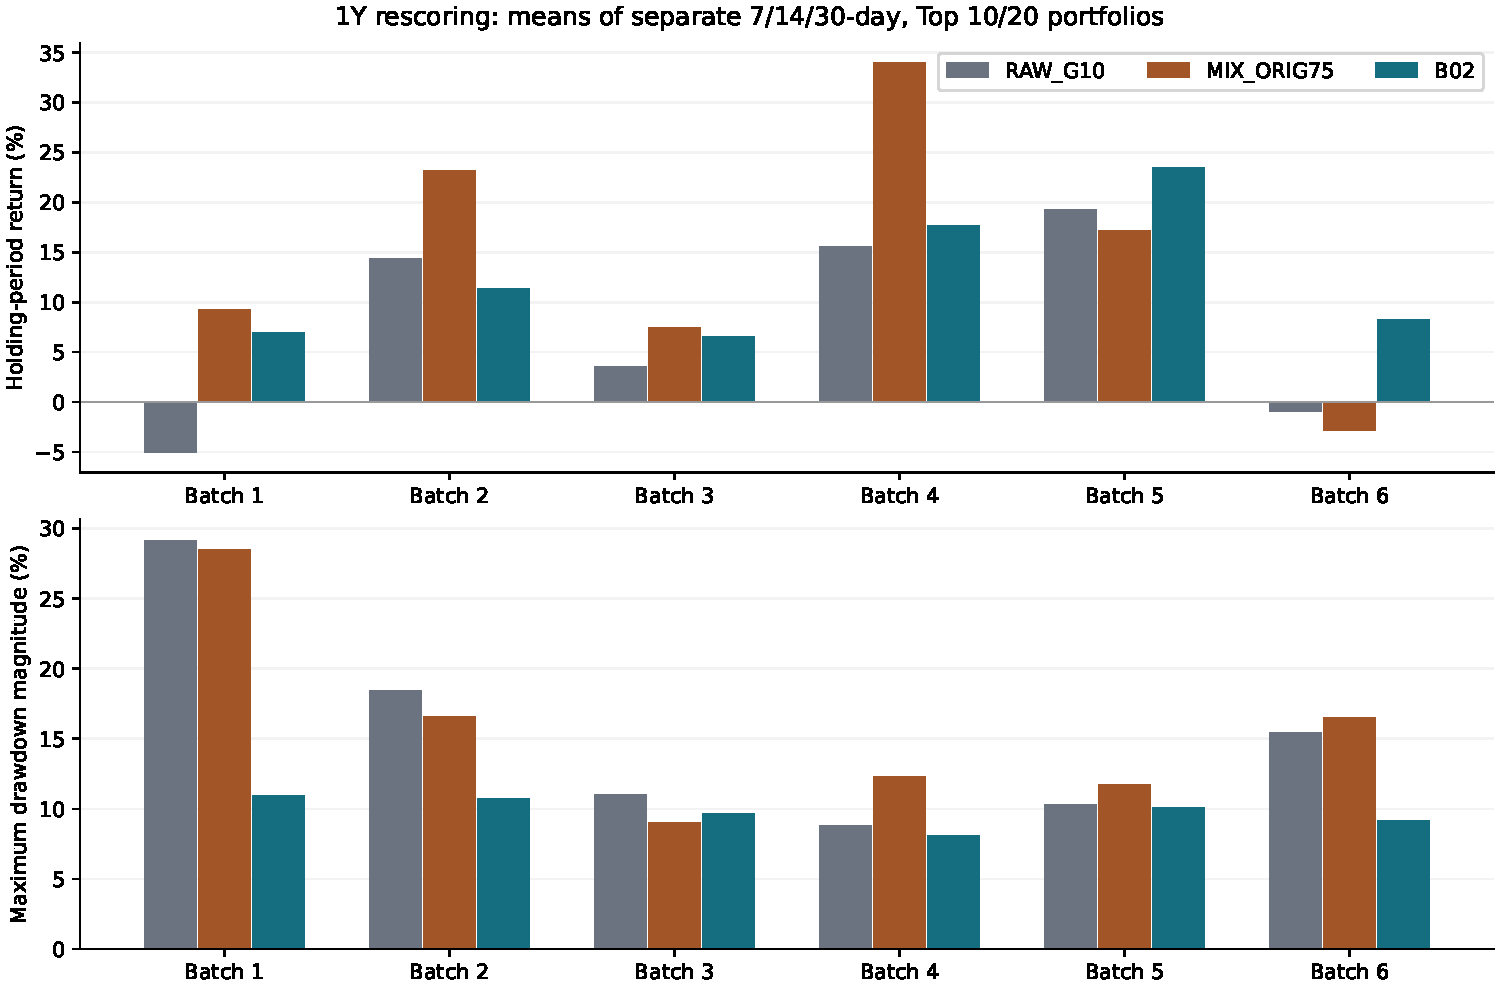
\includegraphics[width=.97\linewidth]{rescoring_comparison.pdf}\caption{One-year rescoring: cohort means across 7-, 14- and 30-day checkpoints and Top 10/20 equal-weight portfolios.}\end{figure}

\subsection{Where the continuity advantage comes from}

The economic mechanism can be traced stock by stock. For each matched
one-year portfolio pair, we identify names selected only by 75/25 and
names selected only by Raw G10, then classify their split-adjusted local
price move from the original anchor to the checkpoint. The subsequent
USD profit contribution of each changed sleeve measures its effect on
the return gap. Shared holdings cancel exactly. The primary Batches 3--5
breakdown is:

\begin{minipage}{\linewidth}
\begin{center}\small\setlength{\tabcolsep}{4pt}\renewcommand{\arraystretch}{1.18}
\begin{longtable}{@{}lrrrrr@{}}\toprule
Lag & Changed slots & Keep risers & Avoid decliners & Other changes & Total gap pp\\\midrule\endhead
7 & 32.5\% & +6.16 & -4.31 & +2.57 & +4.43\\
14 & 39.2\% & +4.79 & -5.60 & +4.82 & +4.00\\
30 & 50.0\% & +12.73 & -4.35 & +3.41 & +11.79\\
All & 40.6\% & +7.89 & -4.75 & +3.60 & +6.74\\
\bottomrule\end{longtable}\end{center}
\end{minipage}\par

The blend's 6.74-point advantage is led by retaining early risers:
blend-only names whose prices had risen contribute +7.89 points. Avoiding
early decliners contributes $-4.75$ points, because the raw-only decliners
subsequently earned positive returns on average. Other selection changes
add +3.60 points. The result supports winner retention as the leading
observed mechanism; it does not support attributing the gain to successful
falling-knife avoidance. Across all six cohorts, the corresponding
contributions are +8.67, $-3.09$ and +1.34 points, summing to +6.92 points.

\subsection{Median outcomes and the common Moderna control}

Cell medians show whether the result extends beyond the mean. Replacing
Moderna with its original allocation held in cash applies the same
issuer-level control to both policies:

\begin{minipage}{\linewidth}
\begin{center}\small\setlength{\tabcolsep}{4pt}\renewcommand{\arraystretch}{1.18}
\begin{longtable}{@{}lrrrrr@{}}\toprule
Scope & Cells & Raw median & 75/25 median & Wins & MRNA cash wins\\\midrule\endhead
Batches 3--5 & 18 & 8.52 & 15.82 & 15/18 & 13/18\\
Batches 1--6 & 36 & 7.24 & 14.37 & 25/36 & 17/36\\
\bottomrule\end{longtable}\end{center}
\end{minipage}\par

The primary-set median rises from 8.52\% to 15.82\%, and the all-cohort
median rises from 7.24\% to 14.37\%. Under the common Moderna-to-cash
control, the blend still wins 13 of 18 primary cells and averages
15.20\% versus Raw G10's 12.80\%. Across all 36 cells, however, it wins
17 and averages 3.32\% versus 4.84\%; the controlled medians are
5.15\% for both after rounding. The primary-cohort improvement therefore
survives this control, while the all-cohort average advantage does not.


\section{Portfolio Accounting, Distributions, and Outlier Sensitivity}

To ensure our empirical comparisons reflect realistic equity ownership rather than idealized index approximations, every simulated portfolio adheres to strict cash-flow and corporate-action accounting:

\textbf{Initial Funding \& Weights:}  Each portfolio starts with USD 100,000 invested in fractional shares at the applicable entry close/open. Original scoring tests both equal weights ($w_i = 1/N$) and linearly declining rank weights ($w_i = 2(N - i + 1)/[N(N + 1)]$); dynamic rescoring uses equal weights exclusively.

\textbf{Corporate Actions, FX, and Gross Distributions:}  Holdings track genuine stock splits and mandatory spin-off child securities (such as Comcast's Versant Media Group spin-off). Non-USD securities (including minor-unit quotes) are valued in USD using dated daily foreign-exchange rates. Actual gross dividends accumulate as uninvested cash on their payment date, while dividends that have gone ex-date prior to the November cutoff but have not yet been paid are tracked separately as earned unpaid receivables (and four unit sleeves with unresolved payment dates totaling at most USD 263.64 in any rescoring portfolio are recorded distinctly).

\textbf{Total Return \& Portfolio Drawdown:}  Terminal wealth $W_{\text{end}}$ equals the market value of equity holdings plus accumulated cash distributions and earned dividend claims, giving percentage return $100(W_{\text{end}} / 100,000 - 1)$. Portfolio maximum drawdown is computed from the combined daily portfolio wealth path with the initial USD 100,000 included in the running peak.

\subsection{The Role of Breakout Outliers: Same-Breadth Moderna Sensitivity}

A defining characteristic of return-focused equity investing is positive skewness: a handful of breakout winners often drive a large share of excess portfolio returns. In our sample, Moderna (MRNA) was a major high-conviction winner selected by G10 (which focuses on upside and discounts model disagreement) but passed over by B02 (which penalized Moderna's high historical price volatility).

To quantify this concentration exposure transparently, we run two diagnostic stress tests without removing genuine winners from our primary tables:

\textbf{Symmetric Best/Worst Sleeve-to-Cash Control:}  Replaces each portfolio's single highest-profit (or lowest-profit) stock sleeve with its initial USD allocation held in zero-interest cash (reported in the final column of Tables 6.1--6.4).

\textbf{Common Moderna-to-Cash Diagnostic:}  Replaces any Moderna position in original-scoring Top 10 equal-weight portfolios with zero-interest cash across both strategies:

\begin{minipage}{\linewidth}
\begin{center}\small\setlength{\tabcolsep}{3pt}\renewcommand{\arraystretch}{1.18}
\begin{longtable}{@{}p{.22\linewidth}rrrr@{}}
\caption{Same-breadth Moderna-to-cash sensitivity (\%)}\\
\toprule
Entry convention & G10 primary & G10 MRNA/cash & B02 primary & B02 MRNA/cash\\\midrule\endhead
Original-Anchor Entry & 31.28 & 6.32 & 11.84 & 11.84\\
Source-Availability Entry & 19.27 & 5.81 & 10.92 & 10.92\\
\bottomrule\end{longtable}\end{center}
\end{minipage}\par
This diagnostic illuminates the core economic trade-off of the paper. G10's higher headline mean return (31.28\% at anchor and 19.27\% at availability) relies heavily on its willingness to back volatile, high-upside outliers like Moderna; when Moderna is replaced by zero-yielding cash without substituting the 11th-ranked stock, G10's six-cohort mean drops to 6.32\% and 5.81\%, whereas B02---which never held Moderna---remains rock-steady at 11.84\% and 10.92\%. Rather than treating Moderna as an "error" to be deleted or claiming G10 is unconditionally superior, this sensitivity shows why offering both a Return-Focused strategy (to capture breakout outliers) and a Risk-Adjusted strategy (to build steady, diversified wealth) is essential.

\subsection{Original-Anchor Terminal Wealth Components (G10 Top 10, B02 Top 20, Equal Weights; End Date: 2 November 2026)}

\begin{minipage}{\linewidth}
\begin{center}\small\setlength{\tabcolsep}{3pt}\renewcommand{\arraystretch}{1.18}
\begin{longtable}{@{}lrrrrrr@{}}
\caption{Terminal wealth and distribution components (USD): G10 Top 10, B02 Top 20}\\
\toprule
Batch & G10 wealth & G10 cash & G10 unpaid & B02 wealth & B02 cash & B02 unpaid\\\midrule\endhead
Batch 1 & 148,389 & 0 & 0 & 150,532 & 2,721 & 417\\
Batch 2 & 137,124 & 516 & 0 & 112,893 & 2,900 & 42\\
Batch 3 & 125,655 & 748 & 0 & 116,806 & 1,632 & 67\\
Batch 4 & 152,948 & 1,247 & 0 & 114,905 & 1,606 & 83\\
Batch 5 & 113,372 & 506 & 97 & 107,134 & 1,110 & 71\\
Batch 6 & 110,186 & 348 & 126 & 111,787 & 547 & 238\\
\bottomrule\end{longtable}\end{center}
\end{minipage}\par
Notice a revealing portfolio dividend pattern in Table 7.2: across every single batch, Risk-Adjusted B02 collects substantially more cash dividends and earned receivables than Return-Focused G10 (e.g., USD 2,721 vs. USD 0 in Batch 1; USD 2,900 vs. USD 516 in Batch 2), because normalizing for historical volatility naturally tilts B02 toward established, dividend-paying companies.

\subsection{The realized dividend-income tilt at matched breadth}

A matched-breadth comparison isolates the dividend pattern from the
Top 10/Top 20 construction choice. Across the six original-anchor cohorts,
mean gross paid distributions as a fraction of initial capital are:

\begin{minipage}{\linewidth}
\begin{center}\small\setlength{\tabcolsep}{4pt}\renewcommand{\arraystretch}{1.18}
\begin{longtable}{@{}lrrrr@{}}\toprule
Breadth & G10 paid yield & B02 paid yield & G10 paid + unpaid & B02 paid + unpaid\\\midrule\endhead
Top 10 & 0.56\% & 2.02\% & 0.60\% & 2.22\%\\
Top 20 & 0.64\% & 1.75\% & 0.67\% & 1.91\%\\
\bottomrule\end{longtable}\end{center}
\end{minipage}\par

At matched Top 10 breadth, B02 collects 2.02\% in paid distributions
versus G10's 0.56\%---about 3.60 times as much---without an additional
dividend factor in Equation 6. Including earned unpaid distributions
raises those figures to 2.22\% and 0.60\%. This observed income tilt
is consistent with selecting more dividend-paying companies through
volatility normalization. These are cumulative holding-period cash yields
on initial capital, averaged equally across the six cohorts.


\section{Production Architecture (Engine V8) and Editorial Governance}

Translating empirical research into a live financial platform requires clear boundaries between original model scores, daily rescoring mechanics, and human/editorial review:

\textbf{Versioned Engine Deployment:}  Under Engine V8, currently eligible 1-year BUY candidates are ranked daily by $\max(0,\, 0.75S_0 + 0.25S_t)$, where $S_0$ is the fixed original G10 score and $S_t$ is the current updated G10 score. Flooring the blend at zero ensures that a historical score cannot manufacture a synthetic negative SELL signal when current fundamentals pass the bullish BUY eligibility guards. Current non-BUY stocks and 5-year rankings retain raw updated G10 ($S_t$). Displayed expected return figures on the platform always show the current mechanical calculation ($R_t$), never a blended return.

\textbf{Cross-Asset Platform Standardization:}  On the iPulse AI platform, the principal G10 ranking architecture is deployed across equities, cryptocurrencies, commodities, foreign exchange, and indices, while B02 serves as the dedicated Risk-Adjusted equity screen. Production verification reconciled both forecast horizons across 426 live assets (3,408 scalar calculations) while keeping all 852 historical rows, 146 published editorial editions, and 28 archives immutable.

\textbf{Transparent Editorial Governance:}  Quantitative rankings and editorial publications maintain strict separation of duties. When editorial reviews evaluate the top-ranked quantitative candidates to assemble a curated ten-pick list, they may select, downgrade, or pass on candidates based on documented qualitative evidence---but they never privately alter the quantitative formula or inject uncalibrated multipliers into G10 or B02. Published comparison tables display selected picks alongside the remaining quantitative candidates with their exact published ranks and explicit review dispositions.

\section{Synthesizing Ranking Continuity with Research Reuse}

How does our 75/25 rescoring breakthrough interact with the broader economic question of when to pay for fresh AI stock research?

In our companion study, When Is Fresh AI Stock Analysis Worth It? (Ramdowar, 2026), we examined a balanced panel of 203 stocks across three cohort transitions (Batches $3\to 4$, $4\to 5$, and $5\to 6$) using a USD 300,000 portfolio, 10-basis-point transaction costs, and a USD 3,000 all-in compute and data bill per fresh deep-research batch. That study showed that over short windows where the underlying AI model architecture was unchanged ($3\to 4$ and $5\to 6$), reusing existing price targets with a historical shock guard generated +2.25\% net return versus +1.66\% for the S\&P 500 ETF (SPY) and +4.24\% for fresh research---whereas over a longer holding window ($3\to 4\text{ long}$), stale research decayed to -11.26\% while fresh research returned +8.55\% (vs. +3.46\% for SPY).

Because the companion study evaluated a specific seven-framework price-forecast council under its historical D3 shock rule, a natural question arises: how much of the gap between reused research and fresh research can be closed simply by upgrading the ranking formula to G10 and our 75/25 continuity blend?

\subsection{Controlled Bridge Experiment: Scoring Both Research Arms on the 203-Stock Panel}

To answer that question on an exact apples-to-apples basis, we applied Raw Updated G10, the 75/25 Continuity Blend, and Risk-Adjusted B02 to both the Reused Research arm and the Fresh Research arm across all 203 stocks (609 forecast councils, 88 independent unit paths, and 792 fee/cost scenarios) under the companion study's exact net-dividend wallet, transaction fees, and USD 3,000 fresh-research charge:

\begin{minipage}{\linewidth}
\begin{center}\small\setlength{\tabcolsep}{3pt}\renewcommand{\arraystretch}{1.18}
\begin{longtable}{@{}lrrrrr@{}}
\caption{Matched Top 10 net holding-period returns (\%)}\\
\toprule
Transition window & Reuse raw & Reuse 75/25 & Fresh raw & Fresh 75/25 & SPY\\\midrule\endhead
Transition $3\to 4$ (Short) & +3.72 & +3.46 & +4.55 & +4.83 & +1.36\\
Transition $4\to 5$ (Short) & +7.42 & +27.16 & +25.86 & +26.97 & +4.47\\
Transition $5\to 6$ (Short) & +6.19 & +8.91 & +6.75 & +6.75 & +1.97\\
Transition $3\to 4$ (Long Window) & -1.57 & -4.23 & +8.55 & +38.36 & +3.46\\
\bottomrule\end{longtable}\end{center}
\end{minipage}\par
Table 9.1: Matched Top 10 net holding-period returns (\%) on a USD 300,000 portfolio after 10 bps entry/exit trading fees and a USD 3,000 incremental research bill on Fresh arms. The bridge experiment yields three high-value insights for AI research platform design:

\textbf{Significant Free Alpha from Better Ranking in Short Windows:} Across the two unchanged-model short windows ($3\to 4$ and $5\to 6$), simply replacing the companion paper's old shock guard (2.25\%) with Raw Updated G10 lifts reused-research return to 4.96\%, and applying the 75/25 Continuity Blend lifts it further to 6.19\%---a marginal gain of +1.23 percentage points from the 75/25 blend alone (and +0.67 percentage points after replacing each portfolio's best stock sleeve with cash: 3.07\% vs. 2.40\%, with neither policy holding Moderna in those two windows). Remarkable in its own right, Reused 75/25 (6.19\%) slightly edges out Fresh Raw G10 (5.65\%) and Fresh 75/25 (5.79\%) net of the USD 3,000 research fee over those short windows, while Risk-Adjusted B02 on reused research averages 7.49\%.

\textbf{Higher Top-10 Shortlist Agreement with Fresh AI Analysis:} Comparing the Top 10 stocks selected from reused forecasts against the Top 10 stocks selected from fresh AI reports (under fixed Fresh Raw G10) shows that the 75/25 continuity blend increases shortlist overlap in every single transition---rising from 2/10, 3/10, and 2/10 under Raw G10 to 3/10, 5/10, and 4/10 under the 75/25 blend---even though full-universe Spearman rank correlation ($\rho$) across all 203 stocks remains broadly similar:

\begin{minipage}{\linewidth}
\begin{center}\small\setlength{\tabcolsep}{3pt}\renewcommand{\arraystretch}{1.18}
\begin{longtable}{@{}lrrrrr@{}}
\caption{Top-10 overlap and full-panel rank agreement}\\
\toprule
Transition & Raw overlap & Blend overlap & Both blended & Raw $\rho$ & Blend $\rho$\\\midrule\endhead
Transition $3\to 4$ & 2/10 & 3/10 & 2/10 & 0.724 & 0.720\\
Transition $4\to 5$ & 3/10 & 5/10 & 4/10 & 0.650 & 0.647\\
Transition $5\to 6$ & 2/10 & 4/10 & 4/10 & 0.685 & 0.704\\
\bottomrule\end{longtable}\end{center}
\end{minipage}\par
Table 9.2: Top-10 shortlist overlap and 203-stock Spearman rank correlation ($\rho$) against the fixed Fresh Raw G10 comparator.

\subsection{Where Score Blending Hits Its Limits: Portfolio Breadth and Thesis Decay}

While the 75/25 continuity blend shines in concentrated Top 10 short-window reuse, Table 9.3 exposes two critical operational boundaries:

\begin{minipage}{\linewidth}
\begin{center}\small\setlength{\tabcolsep}{3pt}\renewcommand{\arraystretch}{1.18}
\begin{longtable}{@{}lrrrrrr@{}}
\caption{Breadth and holding-window sensitivity (\%)}\\
\toprule
Top N & Transition & Reuse raw & Reuse 75/25 & Fresh raw & Fresh 75/25 & Filled slots\\\midrule\endhead
Top 10 & $3\to 4$ (Short) & +3.72 & +3.46 & +4.55 & +4.83 & 10 / 10\\
Top 10 & $4\to 5$ (Short) & +7.42 & +27.16 & +25.86 & +26.97 & 10 / 10\\
Top 10 & $5\to 6$ (Short) & +6.19 & +8.91 & +6.75 & +6.75 & 10 / 10\\
Top 10 & $3\to 4$ (Long) & -1.57 & -4.23 & +8.55 & +38.36 & 10 / 10\\
Top 30 & $3\to 4$ (Short) & +6.28 & +2.27 & +3.91 & +3.41 & 18 / 30\\
Top 30 & $4\to 5$ (Short) & +9.38 & +11.19 & +10.85 & +13.32 & 30 / 30\\
Top 30 & $5\to 6$ (Short) & +3.27 & +2.60 & +1.80 & +1.00 & 30 / 30\\
Top 30 & $3\to 4$ (Long) & +5.51 & -1.87 & +17.21 & +16.54 & 18 / 30\\
\bottomrule\end{longtable}\end{center}
\end{minipage}\par
Table 9.3: Breadth and holding-window sensitivity on the 203-stock research-reuse panel (unfilled slots remain in zero-interest USD cash).

\textbf{Outlier Concentration in Transition $4\to 5$:}  In Transition $4\to 5$, Reused 75/25 jumps to +27.16\% vs. +7.42\% for Raw G10 because the 75/25 blend retained Moderna in the Top 10 while Raw G10 rotated out of it; replacing Moderna's sleeve with cash brings Reused 75/25 to +6.73\% (leaving a +0.59 percentage-point mean advantage for Reused 75/25 across all three short windows under the common Moderna-cash control). Similarly, Fresh 75/25's +38.36\% return in the long window drops to +3.13\% when its Moderna sleeve is held as cash.

\textbf{Breadth Dilution in Top 30:}  When expanding from Top 10 to Top 30, the blended score must still clear the absolute BUY threshold of 130. In Transition $3\to 4$, only 18 of 30 slots pass that hurdle under the 75/25 blend (leaving 12 slots in cash), causing Reused 75/25 to trail Raw G10 in two of the three short Top 30 windows.

\textbf{Ranking Continuity Cannot Fix Stale Fundamentals:}  In the extended holding window ($3\to 4\text{ long}$), both Reused Raw G10 (-1.57\%) and Reused 75/25 (-4.23\%, despite a smaller maximum drawdown of -10.27\% vs. -14.68\%) lose money, whereas commissioning Fresh AI Research delivers +8.55\% (Raw G10) and +17.21\% (Top 30 Raw G10) even after paying the USD 3,000 research fee.

Taken together, the two papers establish a unified operating doctrine for AI investment platforms: use conviction-aware rescoring (75/25 G10) to extract maximum value from concentrated Top 10 picks between research cycles, use B02 when targeting volatility-controlled exposure, and commission fresh multi-agent research when time or material corporate events erode the underlying thesis.

\subsection{What fresh research could afford to cost}

The bridge also gives a concrete research-budget comparison. Let $F$
be the terminal wealth multiple from fresh research before the incremental
research bill, and $U$ the multiple from reused 75/25 research, both after
the same share-trading costs. At portfolio capital $P$, the break-even
research bill is $C^*=P(1-U/F)$. For a USD3,000 bill, minimum capital is
$P^*=3000/(1-U/F)$ when $F>U$. The Top 10 results are:

\begin{minipage}{\linewidth}
\begin{center}\small\setlength{\tabcolsep}{4pt}\renewcommand{\arraystretch}{1.18}
\begin{longtable}{@{}lrrrr@{}}\toprule
Window & Raw: max bill & Raw: min capital & 75/25: max bill & 75/25: min capital\\\midrule\endhead
3$\to$4 short & 6,100 & 147,537 & 6,867 & 131,054\\
4$\to$5 short & None & None & 2,544 & 353,759\\
5$\to$6 short & None & None & None & None\\
3$\to$4 long & 37,965 & 23,706 & 94,437 & 9,530\\
\bottomrule\end{longtable}\end{center}
\end{minipage}\par

Amounts are USD; maximum bills use USD300,000 capital. ``None'' means
fresh research trails reuse even before paying for research, so no positive
bill or portfolio-size break-even exists under proportional scaling.
In the first short window, fresh raw G10 could pay up to USD6,100,
corresponding to about USD147,537 minimum capital for a USD3,000 bill.
In the longer version of that window, the budget rises to USD37,965 and
the minimum capital falls to USD23,706. The very large USD94,437 long-window
budget for fresh 75/25 inherits its Moderna concentration documented above.
These ex-post boundaries make the economic contrast tangible: a stronger
ranking policy can stretch existing research, while a deteriorating thesis
can make fresh evidence worth substantially more.


\section{Conclusion, Methodological Boundaries, and Declarations}

\subsection{Summary of Operating Decisions}

By untangling original forecast scoring from post-publication rescoring---and separating upside maximization from volatility normalization---this study establishes a transparent, versioned ranking architecture for Engine V8:

\textbf{Original Scoring:}  Deploy G10 (Equations 1--5) as the principal Return-Focused formula and B02 (Equation 6) as the dedicated Risk-Adjusted equity formula.

\textbf{Dynamic Rescoring:}  Apply the 75/25 original/updated G10 score blend (Equation 8, $\lambda = 0.75$) subject to current economic BUY guards for 1-year BUY rankings; retain Raw Updated G10 ($\lambda = 0$) for 5-year rankings and non-BUY candidates; and maintain B02 on checkpoint returns and historical volatility for risk-adjusted screening.

\textbf{Research Lifecycle Integration:}  Pair daily price-based rescoring with periodic and event-driven deep research refreshes, recognizing that ranking continuity preserves short-term conviction in concentrated portfolios but cannot substitute for fresh fundamental analysis over extended horizons.

\subsection{Consolidated Methodological Boundaries and Study Limitations}

To keep the main narrative readable while maintaining strict scientific transparency, we consolidate all experimental caveats, statistical boundaries, and accounting disclosures here:

\textbf{Non-Equivalence of Scores, Probabilities, and Realized Ratios:}  Neither G10 nor B02 is a calibrated probability of profit or a forecast percentage return. B02 ($J = (R - 3.6)/\max(v, 5)$) is an ex-ante forecast excess-return-to-historical-volatility ratio, not a realized Sharpe ratio or a guarantee of downside safety. In portfolio evaluation, our Risk-Adjusted comparison metric---holding-period return divided by $\max(\vert{}\text{drawdown}\vert{}, 1)$---is a descriptive within-cell ranking criterion, not an annualized Calmar ratio or a fitted investor utility function.

\textbf{Score Blending Mechanics:}  The 75/25 continuity policy weights original and current G10 scores ($0.75S_0 + 0.25S_t$), never price targets, expected returns, capital allocations, or prior-day blended scores. For legacy cohorts, $S_0$ is reconstructed directly from frozen original inputs via G10; legacy V7 integer scores are never substituted into the blend. Equation 8 alters only ranking order; it does not extend forecast maturity or imply a 75\% probability that an older thesis remains intact.

\textbf{Retrospective Design, Overlapping Windows, and Backtest Overfitting:}  Both the 48-rule original-scoring grid (including its 40-to-20-to-10 descriptive consistency funnel) and the 115-policy rescoring grid (where the 57-policy second round and BUY-screen sensitivities were informed by observing initial round outcomes) are retrospective and partly outcome-informed. Because older cohort portfolios remain invested across later batch anchor dates through the November 2026 cutoffs, holding windows overlap and vary in duration; a 5Y-labelled portfolio reflects selection by the 5-year forecast evaluated over the observed interval through November 2026, not a completed five-year holding period. Accordingly, the 3,456 original portfolios, 8,280 rescoring portfolios, and 792 research-reuse cost scenarios represent computational grid coverage across shared issuers and market windows---not independent statistical trials. Consistent with established literature on multiple-testing bias (Bailey et al., 2015; CFA Institute, 2026), we report descriptive multi-cohort means and cell win rates rather than claiming $p$-values, probabilities of backtest overfitting, or universal out-of-sample optimality.

\textbf{Point-in-Time Data Lineage and Historical Reconstructions:}  In the original-scoring study, Original-Anchor entry is a retrospective counterfactual, whereas Source-Availability entry waits until compatible v2.3 scores were recorded in June/July 2026. Experimental formulas operate on frozen summary inputs (which, due to persisted rounding, cannot replicate every internal historical integer score bit-for-bit, though Batch 6's 694 pre-event values match the v2.3 core exactly and its single stock without the later overlay remains in the cohort). In the rescoring study, all original forecasts pass a generation-before-checkpoint timestamp audit, though stored summary inputs and dividend yield assumptions ($y_0$) were reconstructed retrospectively rather than replaying today's live trailing-dividend service. Original-scoring volatility inputs ($v$) use ten-year raw closing returns (which can be affected by unadjusted splits and are preserved intact for replication), whereas rescoring and live production use corporate-action-adjusted daily return series requiring at least 60 prior observations (excluding only recent listing SPCX in Batch 6, which had 21/26/38 observations at the three checkpoints, affecting 6 horizon-checkpoint records).

\textbf{Trading Friction, Taxes, and Cross-Study Comparability:}  In the USD 100,000 original-scoring and rescoring studies, portfolios execute no post-entry discretionary trades, dividend reinvestments, cash interest accruals, brokerage fees, bid-ask spreads, market impact, leverage, or tax withholdings (whereas the USD 300,000 bridge experiment in Section 9 explicitly applies the companion study's 10-bps trading fees, net dividend wallet, and USD 3,000 fresh-research charge on a controlled 7-framework price-only council rather than a full 14-advisor native V8 replay). Cross-asset deployment of G10 to crypto, commodities, forex, and indices is an approved methodology extension beyond the equity-only empirical evidence presented here. Similarly, the companion paper's reference to the "production D3 rule" reflects the historical D3 shock rule active prior to the 4 November 2026 V8 update.

\subsection{Declarations}

The author develops and operates the iPulse AI platform through Future Edge Group FZE and holds a commercial interest in its research technology. This manuscript utilized AI-assisted analysis, code generation, drafting, and verification; the named author assumes full responsibility for the final work. All computational checks and source artifacts are retained in the private author replication archive. Licensed upstream market data remain subject to their respective vendor agreements independently of any license applied to the manuscript or authored code.

\appendix
\section{Complete Original Configuration Family (48 Rules)}

The complete 48-rule configuration manifest and executable Python definitions are preserved in frozen\_design.json and scoring.py. The 32-rule core binary factorial toggles five flags $(V, M, A, D, H)$ corresponding to historical volatility ($V$), mean absolute forecast deviation ($M$), directional consistency ($A$), forecast dispersion ($D$), and a 20\% five-year horizon blend ($H$). In this binary notation, G10 corresponds to $(0, 1, 0, 1, 0)$.Let $E$ denote excess return incorporating the MAD discount (Equation 2) when $M = 1$, or simple excess return $R - 3.6$ when $M = 0$. When $V = 0$, the core signal is $E / 15$; when $V = 1$, the core signal bundles a volatility ratio with a soft volatility-scaling denominator:

\begin{equation}\text{signal}_{V=1} = 0.35\frac{E}{\max(v,\, 5)} + 0.65\frac{E}{15a}, \quad a = 1 + \operatorname{clip}\left(\frac{v - 30}{50},\, 0,\, 1\right) \end{equation}

The resulting signal is transformed via $1000\tanh(\text{signal} / 2)$, multiplied by $(0.85 + 0.15C)$ when $A = 1$, and multiplied by $(1 - P)$ when $D = 1$. Setting $H = 1$ combines 80\% of the 1-year core score with 20\% of the corresponding 5-year core score.

The 16 non-factorial benchmark and mechanism-check configurations are defined as follows:

\textbf{B01:}  Ranks purely by expected total return $R$.

\textbf{B02:}  Ranks by the risk-adjusted ratio $(R - 3.6) / \max(v, 5)$ (Equation 6).

\textbf{B03:}  Uses the exact stored historical integer core score.

\textbf{B04:}  Ranks by $R - M$.

\textbf{B05:}  Ranks by $R - s$.

\textbf{B06:}  Ranks by $(R - 3.6)(0.5 + 0.5A_{\text{vote}})$.

\textbf{B07:}  Subtracts 25\% of the absolute stored 1Y/5Y score difference from the stored 1Y score.

\textbf{B08:}  Weights within-batch percentile ranks of expected return (45\%), forecast Sharpe (20\%), negative MAD (15\%), directional vote agreement (10\%), and stored 5Y score (10\%).

\textbf{L10, L20, L35:}  Retain G10 disagreement settings and add direct forecast-Sharpe weights of 0.10, 0.20, and 0.35 without the old volatility anchor multiplier.

\textbf{L10C:}  Adds the consistency multiplier to L10.

\textbf{L10A:}  Adds a softer volatility anchor rising linearly from 1.0 to 1.25 over $v \in [30\%, 80\%]$.

\textbf{A00:}  Applies that soft volatility anchor alone to G10.

\textbf{E25:}  Divides positive G10 scores by $(\max(v, 20) / 20)^{0.25}$ while leaving negative scores unchanged.

\textbf{HNEG:}  Multiplies signed G10 by $1 - 0.10\operatorname{clip}(-S_{5,\text{stored}} / 1000,\, 0,\, 1)$. Because this multiplier shrinks negative 1Y scores toward zero when the 5Y score is negative without altering positive Top 10 selections, it ties G10 at the top of the cohort rankings and is retained solely as a disclosed mechanism check.

\section{Corporate-Action, Cash-Flow, and Quote-Continuity Corrections}

Market-data supplements are maintained as auditable overlays separate from raw vendor exports:

\textbf{Mandatory Spin-Offs:}  Comcast Corporation's separation of Versant Media Group, Inc. (5 January 2026) distributed 1 Versant child share for every 25 parent shares held; simulated portfolios retain the distributed child shares and track their subsequent prices and dividends.

\textbf{Subscription Rights vs. Stock Splits:}  Worldline's rights issue (12 March 2026) required additional cash subscription and is properly treated as an unexercised rights offering under our zero-additional-trading convention rather than a free stock split. Genuine reverse stock splits are reflected directly in share quantities.

\textbf{Adyen Quote-Continuity Bridge:}  Preserves the identical EUR ordinary share and ISIN across its continuing trading venue so that original entry quantities and forecasts remain unbroken. While the initial rescoring run bridged terminal valuation correctly, a forward correction restored two missing dated checkpoint quotes and historical volatility observations in Batch 6.

\section{Complete Cell-by-Cell Rescoring Results Across Checkpoints and Breadths}
\label{app:rescoring-cells}

Each row below represents an independent USD 100,000 equal-weight portfolio entered at the first local market open following the stated 7-, 14-, or 30-day checkpoint and held through 3 November 2026 under the published economic BUY screen. Batches 3--5 constitute the primary evaluation set; Batches 1, 2, and 6 are additional cohorts.

\Needspace{24\baselineskip}
\subsection{1-Year Forecast Selection --- Top 10, Equal Weights}

\begin{minipage}{\linewidth}
\begin{center}\footnotesize\setlength{\tabcolsep}{3pt}\renewcommand{\arraystretch}{1.12}
\begin{longtable}{@{}lrrrrrrr@{}}
\caption{1Y, Top 10 checkpoint results (\%)}\\
\toprule
Batch & Lag & Raw R & Raw DD & 75/25 R & 75/25 DD & B02 R & B02 DD\\\midrule\endhead
1 & 7 & -6.41 & -20.45 & 39.97 & -24.25 & 11.13 & -8.83\\
1 & 14 & -14.64 & -28.55 & 35.46 & -24.96 & 5.38 & -7.51\\
1 & 30 & -19.50 & -40.58 & -34.49 & -45.51 & 1.09 & -18.01\\
2 & 7 & 4.37 & -28.43 & 5.34 & -27.34 & 16.38 & -8.62\\
2 & 14 & 32.52 & -22.74 & 31.75 & -22.01 & 13.18 & -14.56\\
2 & 30 & 5.12 & -14.95 & 36.90 & -12.24 & 4.97 & -11.52\\
3 & 7 & -5.11 & -13.27 & 10.29 & -8.72 & 1.86 & -10.09\\
3 & 14 & 1.68 & -14.97 & 3.59 & -11.17 & 1.00 & -10.83\\
3 & 30 & 5.19 & -11.97 & 6.84 & -10.83 & 16.18 & -9.09\\
4 & 7 & 11.56 & -11.15 & 27.21 & -15.95 & 13.84 & -10.92\\
4 & 14 & 23.28 & -7.19 & 39.66 & -19.68 & 25.40 & -9.26\\
4 & 30 & 7.28 & -6.37 & 44.65 & -8.60 & 15.28 & -7.24\\
5 & 7 & 8.72 & -13.65 & 12.60 & -13.09 & 19.88 & -12.14\\
5 & 14 & 32.68 & -12.10 & 30.36 & -13.17 & 37.68 & -11.12\\
5 & 30 & 15.45 & -7.41 & 19.04 & -12.33 & 17.67 & -9.19\\
6 & 7 & 5.96 & -14.73 & 5.20 & -20.75 & 10.99 & -13.13\\
6 & 14 & -13.47 & -23.85 & 4.51 & -20.60 & 9.27 & -9.12\\
6 & 30 & -0.14 & -14.32 & -14.94 & -17.82 & 7.85 & -5.44\\
\bottomrule\end{longtable}\end{center}
\end{minipage}\par
\Needspace{24\baselineskip}
\subsection{1-Year Forecast Selection --- Top 20, Equal Weights}

\begin{minipage}{\linewidth}
\begin{center}\footnotesize\setlength{\tabcolsep}{3pt}\renewcommand{\arraystretch}{1.12}
\begin{longtable}{@{}lrrrrrrr@{}}
\caption{1Y, Top 20 checkpoint results (\%)}\\
\toprule
Batch & Lag & Raw R & Raw DD & 75/25 R & 75/25 DD & B02 R & B02 DD\\\midrule\endhead
1 & 7 & 26.61 & -17.71 & 16.14 & -20.11 & 7.07 & -9.72\\
1 & 14 & 0.29 & -30.38 & 19.61 & -20.16 & 6.55 & -5.72\\
1 & 30 & -16.94 & -37.39 & -20.82 & -36.00 & 10.65 & -16.03\\
2 & 7 & 8.43 & -18.77 & 21.03 & -14.95 & 14.75 & -7.31\\
2 & 14 & 20.93 & -11.65 & 20.98 & -14.54 & 7.83 & -9.38\\
2 & 30 & 14.76 & -14.31 & 23.01 & -8.61 & 11.05 & -12.87\\
3 & 7 & 7.62 & -5.15 & 7.73 & -6.95 & 3.62 & -8.19\\
3 & 14 & 3.83 & -11.06 & 5.10 & -8.61 & 4.70 & -9.33\\
3 & 30 & 8.33 & -9.52 & 11.22 & -7.67 & 12.13 & -10.27\\
4 & 7 & 16.85 & -8.56 & 19.18 & -11.87 & 17.65 & -6.17\\
4 & 14 & 27.03 & -11.00 & 43.85 & -11.21 & 19.98 & -6.82\\
4 & 30 & 7.21 & -8.70 & 29.55 & -6.46 & 13.91 & -8.25\\
5 & 7 & 19.82 & -10.75 & 9.00 & -10.90 & 20.83 & -10.58\\
5 & 14 & 32.94 & -10.28 & 22.89 & -9.99 & 26.10 & -10.12\\
5 & 30 & 6.12 & -7.87 & 9.02 & -10.92 & 19.00 & -7.52\\
6 & 7 & 1.03 & -13.23 & 0.81 & -14.00 & 8.67 & -12.66\\
6 & 14 & -9.57 & -19.51 & -1.01 & -11.84 & 9.36 & -9.30\\
6 & 30 & 10.26 & -6.89 & -11.95 & -13.98 & 3.30 & -5.20\\
\bottomrule\end{longtable}\end{center}
\end{minipage}\par
\Needspace{24\baselineskip}
\subsection{5-Year Forecast Selection --- Top 10, Equal Weights}

\begin{minipage}{\linewidth}
\begin{center}\footnotesize\setlength{\tabcolsep}{3pt}\renewcommand{\arraystretch}{1.12}
\begin{longtable}{@{}lrrrrrrr@{}}
\caption{5Y, Top 10 checkpoint results (\%)}\\
\toprule
Batch & Lag & Raw R & Raw DD & 75/25 R & 75/25 DD & B02 R & B02 DD\\\midrule\endhead
1 & 7 & 40.96 & -27.91 & 39.50 & -32.16 & 3.09 & -8.66\\
1 & 14 & 35.96 & -34.86 & 36.80 & -33.92 & -1.48 & -15.22\\
1 & 30 & -25.31 & -54.00 & 34.22 & -35.35 & -5.68 & -19.72\\
2 & 7 & 30.04 & -20.56 & 32.99 & -16.64 & 7.95 & -8.05\\
2 & 14 & 22.69 & -21.87 & 32.85 & -15.65 & 5.77 & -10.92\\
2 & 30 & 30.05 & -14.47 & 23.38 & -16.14 & 0.20 & -10.47\\
3 & 7 & -7.43 & -22.65 & -8.83 & -22.81 & 2.49 & -4.93\\
3 & 14 & -3.20 & -18.99 & -6.74 & -21.66 & 4.65 & -7.93\\
3 & 30 & -4.97 & -14.35 & -6.23 & -21.65 & 9.86 & -7.93\\
4 & 7 & 14.74 & -13.55 & 38.67 & -18.36 & 10.39 & -8.02\\
4 & 14 & 61.32 & -10.02 & 57.67 & -14.32 & 17.53 & -5.92\\
4 & 30 & 44.44 & -9.94 & 46.92 & -14.44 & 10.19 & -7.44\\
5 & 7 & -7.62 & -19.31 & -8.68 & -17.58 & 5.73 & -10.93\\
5 & 14 & 18.98 & -13.00 & -5.52 & -17.63 & 15.74 & -12.78\\
5 & 30 & 3.28 & -12.94 & -6.30 & -17.98 & 18.55 & -8.51\\
6 & 7 & -22.72 & -27.53 & -7.71 & -16.38 & 13.28 & -10.24\\
6 & 14 & -18.05 & -30.29 & -10.78 & -22.13 & 6.06 & -8.18\\
6 & 30 & -22.82 & -27.37 & -23.38 & -27.33 & -5.31 & -10.78\\
\bottomrule\end{longtable}\end{center}
\end{minipage}\par
\Needspace{24\baselineskip}
\subsection{5-Year Forecast Selection --- Top 20, Equal Weights}

\begin{minipage}{\linewidth}
\begin{center}\footnotesize\setlength{\tabcolsep}{3pt}\renewcommand{\arraystretch}{1.12}
\begin{longtable}{@{}lrrrrrrr@{}}
\caption{5Y, Top 20 checkpoint results (\%)}\\
\toprule
Batch & Lag & Raw R & Raw DD & 75/25 R & 75/25 DD & B02 R & B02 DD\\\midrule\endhead
1 & 7 & 10.78 & -22.57 & 5.09 & -27.35 & -0.86 & -8.18\\
1 & 14 & 11.70 & -27.19 & 8.00 & -27.81 & 0.87 & -9.99\\
1 & 30 & 11.66 & -29.16 & 10.10 & -28.65 & -3.24 & -14.41\\
2 & 7 & 17.55 & -17.96 & 15.54 & -14.79 & 12.30 & -5.46\\
2 & 14 & 12.84 & -19.04 & 15.23 & -15.69 & 5.79 & -7.65\\
2 & 30 & 13.75 & -14.92 & 9.95 & -15.15 & 6.72 & -9.05\\
3 & 7 & -3.52 & -13.82 & 0.53 & -15.58 & 4.49 & -6.75\\
3 & 14 & -3.32 & -13.69 & 1.77 & -15.37 & 9.97 & -7.04\\
3 & 30 & 0.49 & -10.69 & 2.48 & -14.95 & 12.32 & -6.75\\
4 & 7 & 24.23 & -9.44 & 22.77 & -12.61 & 10.35 & -7.20\\
4 & 14 & 43.43 & -12.14 & 35.52 & -10.88 & 10.35 & -8.04\\
4 & 30 & 26.00 & -9.33 & 25.65 & -7.16 & 9.90 & -6.58\\
5 & 7 & 3.16 & -10.93 & 19.03 & -7.31 & 9.09 & -10.27\\
5 & 14 & 8.89 & -11.11 & 15.15 & -9.59 & 18.08 & -8.93\\
5 & 30 & -3.36 & -12.70 & 8.26 & -11.42 & 11.63 & -8.12\\
6 & 7 & -21.73 & -25.58 & 1.03 & -13.10 & 9.59 & -10.66\\
6 & 14 & -18.81 & -28.45 & -0.71 & -15.20 & 8.82 & -9.45\\
6 & 30 & -6.53 & -20.19 & -11.04 & -15.77 & -3.58 & -11.25\\
\bottomrule\end{longtable}\end{center}
\end{minipage}\par
\section{Reproduction, Validation, and Artifact Provenance}

The 7-rule pilot, 40-rule factorial study, 48-rule original-scoring grid, 115-policy rescoring study, and 203-stock research-reuse bridge extension are maintained in separate sibling directories within the private replication bundle. Raw database exports, read-only SQL queries, timestamp audits, formula manifests, selected rankings, position-level allocations, and daily wealth paths are preserved intact.

The automated build script (build\_final\_manuscript.py) generates all tables and figures directly from the frozen portfolio records, performing an independent arithmetic verification across all 11,736 terminal portfolios and 2,135,172 daily portfolio observations (covering 69,120 original-scoring position allocations and 124,200 rescoring allocations across 1,076 unique unit sleeves), with cryptographic source hashes recorded in paper/calculation\_audit.json. In the 203-stock bridge extension, all 480 retained cost scenarios reconcile within USD $2.92 \times 10^{-10}$, and all 88 unit paths reconcile within USD $7.28 \times 10^{-11}$. The prior 3 November 2026 draft (which proposed B02 as the public default) is preserved in paper/archive\_2026-11-03/.

\begin{thebibliography}{9}
\bibitem{fresh} Ramdowar, R. (2026). \emph{When Is Fresh AI Stock Analysis
Worth It? Allocating a Limited Research Budget Across Price Updates,
Deep Forecast Refreshes, and Editorial Reviews of Top Stock Picks}.
Version 2.1.0, 4 November 2026. Future Edge Group FZE.
\url{https://doi.org/10.5281/zenodo.23941195}.
\url{https://github.com/TheFutureEdge/research-when-fresh-ai-stock-analysis-is-worth-it/releases/tag/v2.1.0}.
\bibitem{bailey} Bailey, D. H., Borwein, J. M., L\'opez de Prado, M., and
Zhu, Q. J. (2015). \emph{The Probability of Backtest Overfitting}.
Revised February 2015. \url{https://www.davidhbailey.com/dhbpapers/backtest-prob.pdf}.
\bibitem{cfa} CFA Institute (2026). \emph{Backtesting and Simulation}.
Level II Portfolio Management refresher reading.
\url{https://www.cfainstitute.org/insights/professional-learning/refresher-readings/2026/backtesting-and-simulation}.
\bibitem{comcast} Comcast Corporation (5 January 2026).
\emph{Comcast Announces Completion of Separation of Versant Media Group, Inc.}
Issuer announcement, SEC Exhibit 99.1.
\url{https://www.sec.gov/Archives/edgar/data/1166691/000095010326000079/dp239108_ex9901.htm}.
\bibitem{worldline} Worldline (12 March 2026).
\emph{Launch of the Rights Issue}.
\url{https://worldline.com/en/home/top-navigation/media-relations/press-release/pr-2026_03_12_02}.
\end{thebibliography}
\end{document}